\documentclass[11pt]{article}

\usepackage[margin=1in]{geometry}
\usepackage{amsmath}
\usepackage{booktabs}
\usepackage{float}
\usepackage{graphicx}
\usepackage[hidelinks]{hyperref}

\setlength{\parindent}{0pt}
\setlength{\parskip}{6pt}
\renewcommand{\arraystretch}{1.15}

\title{Computer Architecture HW4: Introduction to GPU}
\author{Group: TODO}
\date{June 2026}

\begin{document}
\maketitle

\section{Overview}

For this homework I implemented the 2D heat equation on the CPU and on the GPU.
The boundary condition is simple: the top side is fixed at temperature 100, and
the other three sides are fixed at 0. The inside of the plate starts at 0. The
two top corners are set to 50 because they touch one hot side and one cold side.

All versions use row-major arrays and the same update rule:
\[
T_{i,j}^{n+1} =
T_{i,j}^{n} +
r \left(T_{i-1,j}^{n}+T_{i+1,j}^{n}
+T_{i,j-1}^{n}+T_{i,j+1}^{n}-4T_{i,j}^{n}\right).
\]
I used \(r=\alpha \Delta t/h^2=0.24\), which is below the stability limit
\(r \le 0.25\).

The CPU code is the reference solution. The CUDA programs copy the initial grid
to the GPU, run all time steps there, swap the two device arrays after each
step, and only copy the final grid back to the host.

\section{Platform}

The measurements in this report were taken on the following machine.

\begin{center}
\begin{tabular}{ll}
\toprule
Item & Value \\
\midrule
CPU & AMD Ryzen 9 7940H, 8 cores / 16 threads \\
GPU & NVIDIA GeForce RTX 4060 Laptop GPU \\
CUDA compute capability & 8.9 \\
SM count & 24 \\
Max threads per block & 1024 \\
Shared memory per block & 48 KB \\
Shared memory per SM & 100 KB \\
Approx. peak FP32 & 13824.00 GFLOP/s \\
Approx. memory bandwidth & 256.03 GB/s \\
Compiler & \texttt{nvcc 12.0 -O3 -arch=sm\_89}, \texttt{g++ -O3} \\
\bottomrule
\end{tabular}
\end{center}

\section{Arithmetic Intensity}

For one update of an interior grid point, I counted the following operations.

\begin{center}
\begin{tabular}{lr}
\toprule
Work & Count \\
\midrule
Add the four neighbors & 3 additions \\
Compute \(4T_{i,j}\) & 1 multiplication \\
Subtract \(4T_{i,j}\) & 1 subtraction \\
Multiply by \(r\) & 1 multiplication \\
Add the old center value & 1 addition \\
\midrule
Total & 7 FLOPs \\
\bottomrule
\end{tabular}
\end{center}

Without assuming cache reuse, each update reads five floats and writes one
float:
\[
6 \times 4 = 24 \text{ bytes/update}.
\]
So the arithmetic intensity is
\[
I = 7/24 = 0.292 \text{ FLOP/byte}.
\]

For my GPU, the ridge point is
\[
I_{\text{ridge}} = 13824.00/256.03 = 53.99 \text{ FLOP/byte}.
\]
Since \(0.292\) is much smaller than \(53.99\), this stencil is memory-bound.

\section{Part 0: Serial Solver}

The serial code is in \texttt{heat\_serial.cpp}. It is a single-threaded 2D
solver and is also used to check the CUDA output. For the stationary plot I ran
\(N=256\) until the maximum update was below \(10^{-4}\). It stopped after
46941 steps, with final maximum update \(9.918213\times 10^{-5}\).

\begin{figure}[H]
\centering
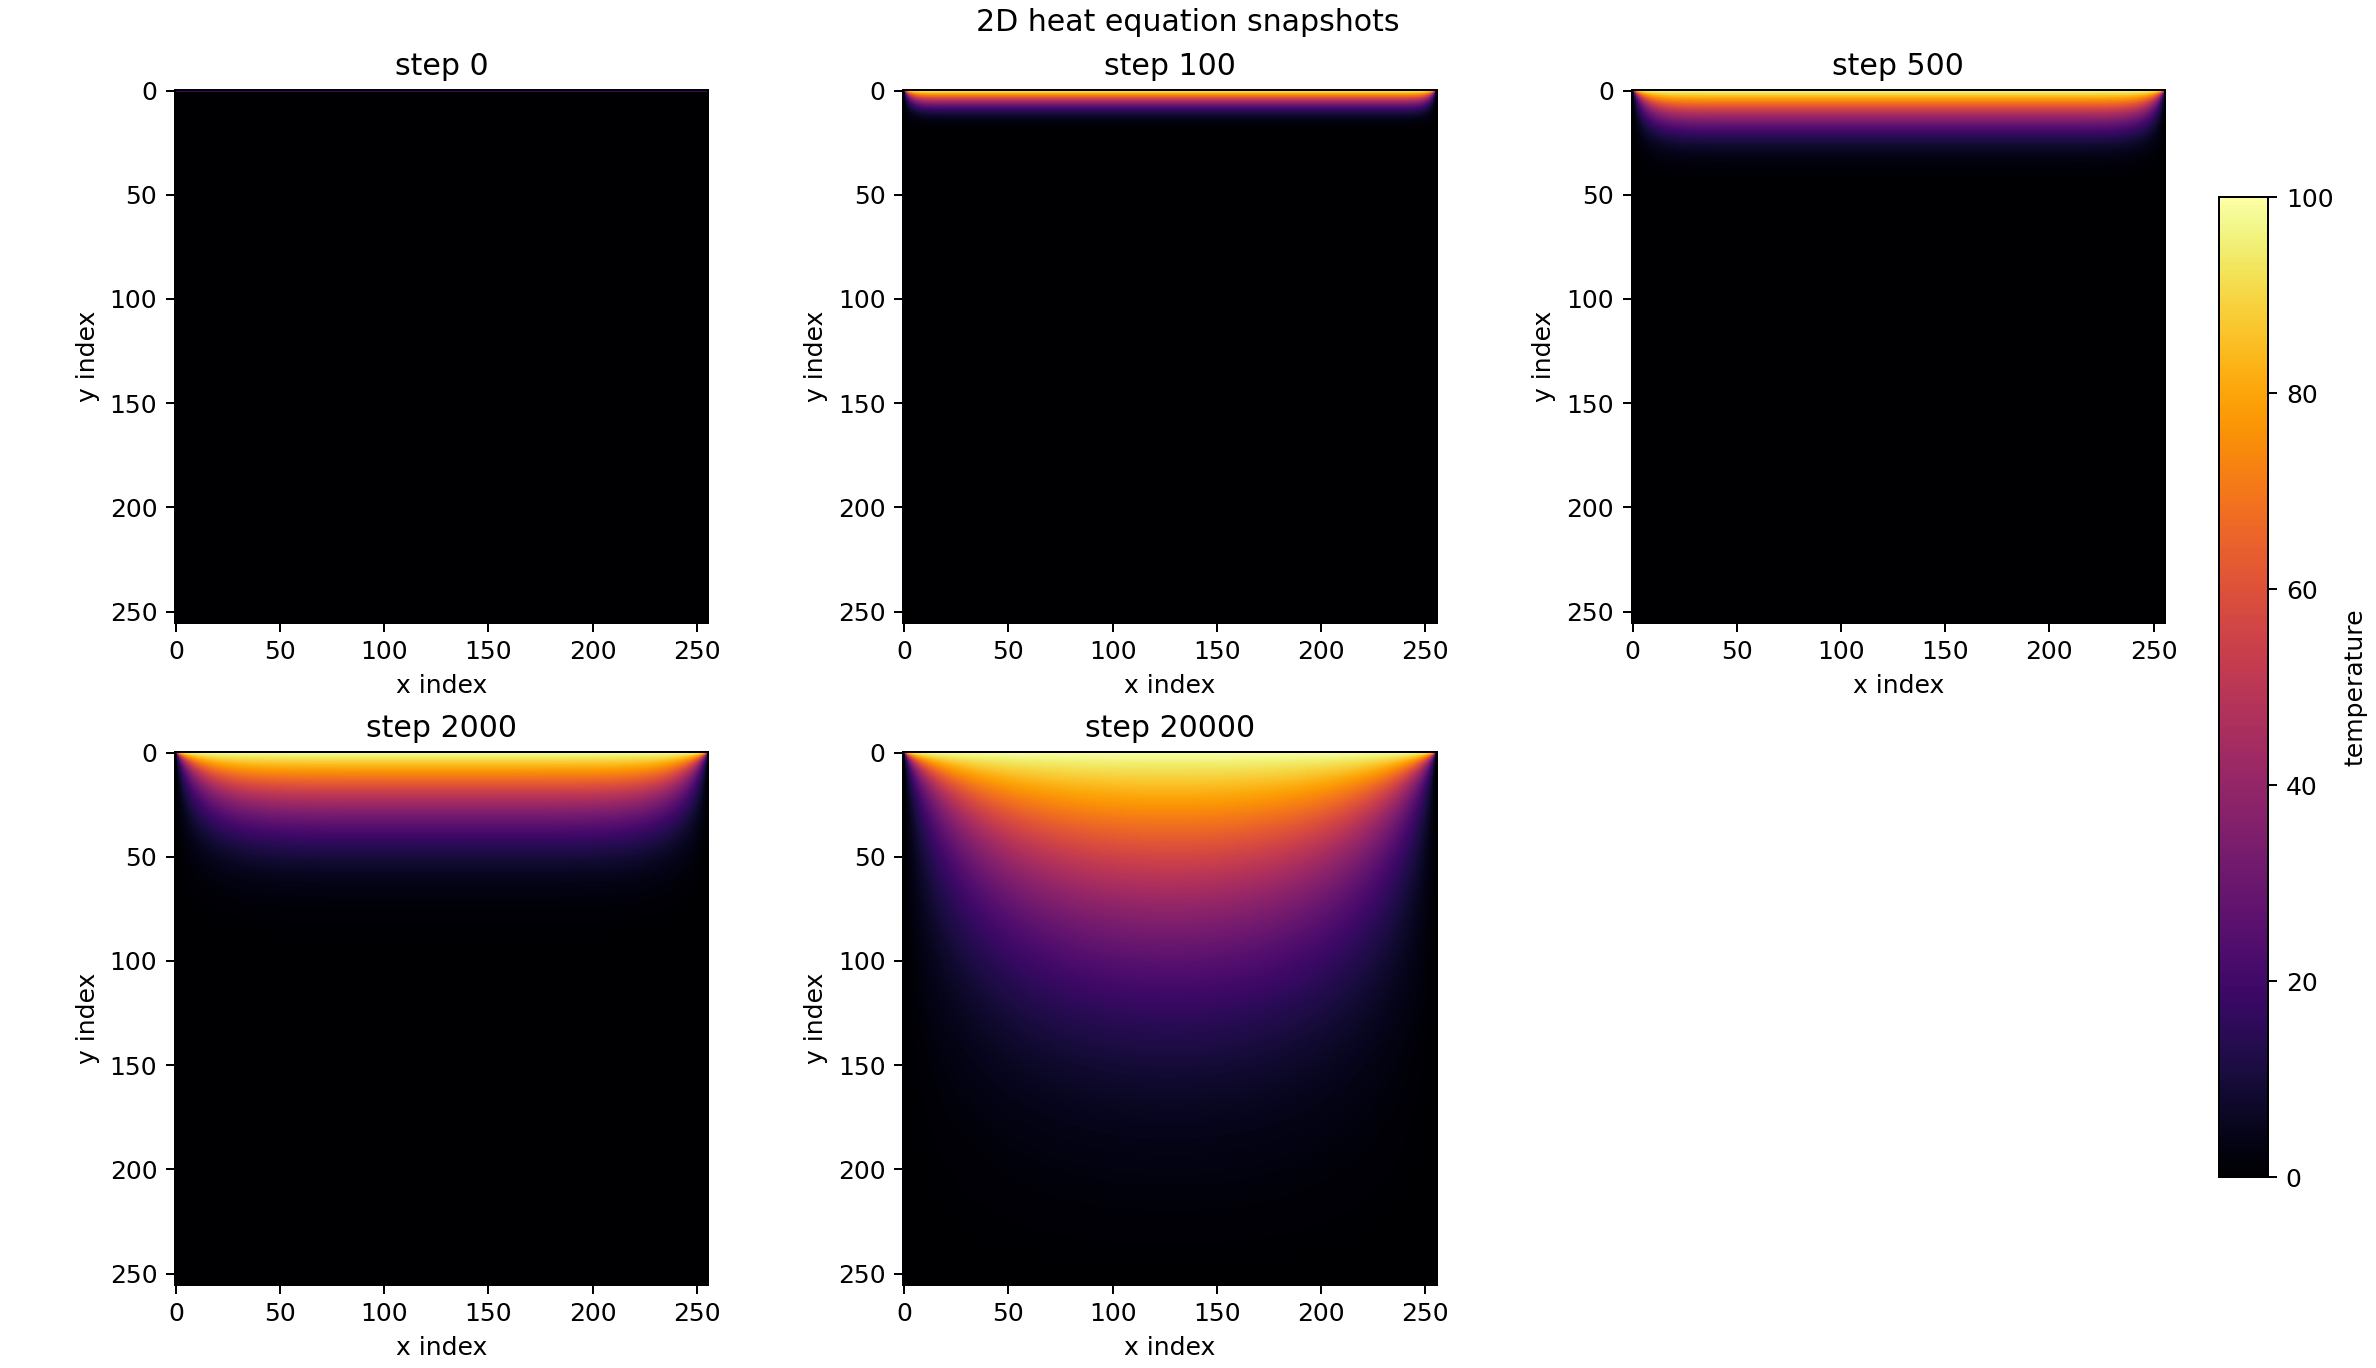
\includegraphics[width=0.95\linewidth]{plots/serial_snapshots.png}
\caption{Serial solution at several time steps.}
\end{figure}

\begin{figure}[H]
\centering
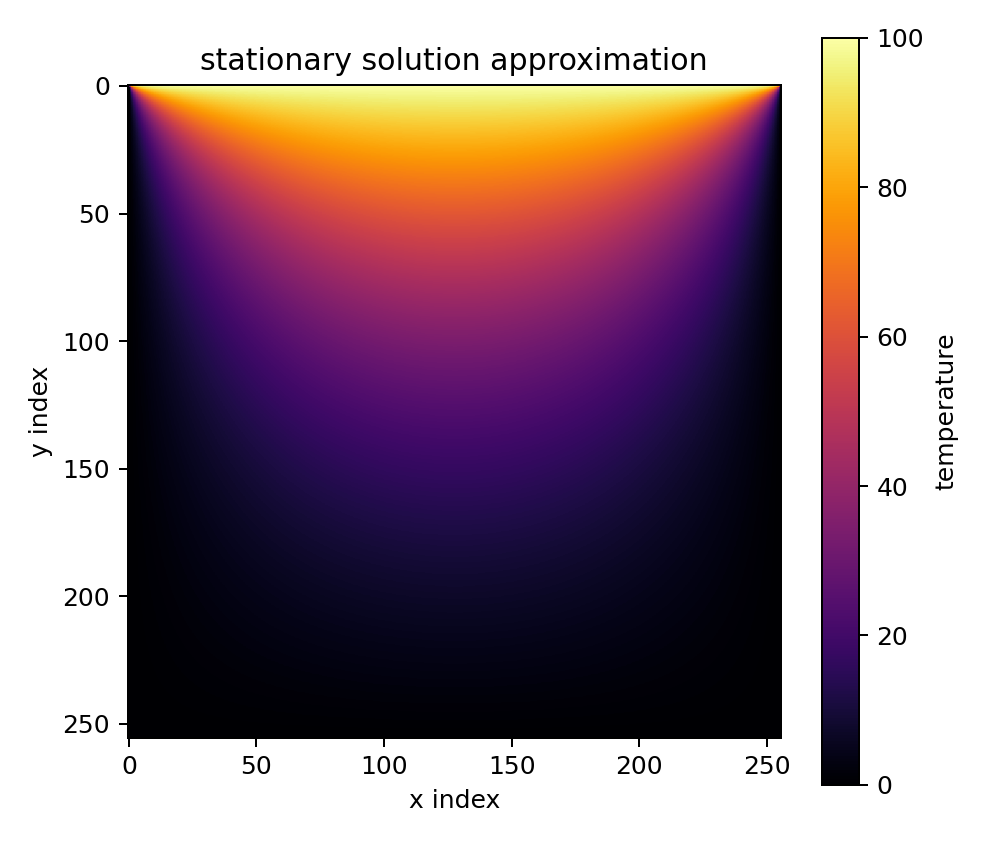
\includegraphics[width=0.70\linewidth]{plots/stationary_solution.png}
\caption{Approximate stationary solution for \(N=256\).}
\end{figure}

The serial timings used for speedup comparisons are:

\begin{center}
\begin{tabular}{rrrr}
\toprule
\(N\) & Steps & Time (ms) & Throughput (Gpt/s) \\
\midrule
512 & 2000 & 980.742 & 0.530 \\
1024 & 2000 & 3843.741 & 0.543 \\
2048 & 2000 & 15809.768 & 0.530 \\
\bottomrule
\end{tabular}
\end{center}

\section{Part A: Naive CUDA Kernel}

The naive CUDA code is in \texttt{heat\_cuda.cu}. Each thread updates one
interior grid point using values from global memory. At \(N=256\), 500 steps,
and block size \(16\times16\), the maximum difference from the CPU result was
\(3.814697\times10^{-6}\).

For convergence checking I used \texttt{thrust::reduce}. On checking steps, the
kernel writes the absolute change of each point into a device array. Then Thrust
finds the maximum value on the GPU. This avoids copying the whole grid back to
the CPU every time step.

\subsection{Block Size Test}

All runs in this table used \(N=1024\) and 2000 steps.

\begin{center}
\begin{tabular}{rrrr}
\toprule
Block size & Threads/block & Time (ms) & Throughput (Gpt/s) \\
\midrule
\(8\times8\) & 64 & 58.312 & 35.824 \\
\(16\times16\) & 256 & 62.867 & 33.228 \\
\(32\times32\) & 1024 & 59.460 & 35.132 \\
\bottomrule
\end{tabular}
\end{center}

The best result here was \(8\times8\). Very small blocks can waste time because
there are more blocks to schedule. Very large blocks can also be worse because
they reduce how many blocks can stay active on one SM. The \(32\times32\) case
has 1024 threads, which is legal on this GPU, but it is exactly the maximum
allowed number.

Using the \(8\times8\) result, the effective bandwidth requested in the
assignment is
\[
BW_{\text{achieved}} =
\frac{(1024-2)^2 \times 24}{58.312\text{ ms}/2000}
= 859.8 \text{ GB/s}.
\]
This is higher than the listed DRAM bandwidth because this formula counts
24 bytes per update as if there were no cache reuse. In practice, nearby
threads reuse data through the GPU caches.

\subsection{Speedup Over Serial}

\begin{center}
\begin{tabular}{rrrr}
\toprule
\(N\) & Serial time (ms) & Naive CUDA time (ms) & Speedup \\
\midrule
512 & 980.742 & 55.376 & 17.71x \\
1024 & 3843.741 & 58.312 & 65.92x \\
2048 & 15809.768 & 255.980 & 61.76x \\
\bottomrule
\end{tabular}
\end{center}

\section{Part B: Shared-memory Kernel}

The tiled version is in \texttt{heat\_cuda\_tile.cu}. Each block first loads a
tile plus a one-cell halo into shared memory. After \texttt{\_\_syncthreads()},
the stencil reads from shared memory instead of reading all neighbors directly
from global memory. At \(N=256\), 500 steps, and tile size \(16\times16\), the
maximum difference from the CPU result was also \(3.814697\times10^{-6}\).

This halo idea is similar to the MPI halo exchange from the previous homework.
In MPI, neighboring processes exchange boundary rows or columns through the
network. In this CUDA version, each thread block loads the needed boundary cells
from global memory into shared memory. The CUDA version has lower latency, but
it still needs careful indexing and a block synchronization.

\subsection{Tile Size Test}

All runs in this table used \(N=1024\) and 2000 steps. The speedup column is
relative to the best naive result from Part A.

\begin{center}
\begin{tabular}{rrrrr}
\toprule
Tile size & Time (ms) & Throughput (Gpt/s) & Speedup & Shared mem/block (KB) \\
\midrule
\(8\times8\) & 105.182 & 19.861 & 0.554x & 0.391 \\
\(16\times16\) & 90.313 & 23.130 & 0.646x & 1.266 \\
\(32\times32\) & 127.187 & 16.424 & 0.458x & 4.516 \\
\bottomrule
\end{tabular}
\end{center}

The GPU has 100 KB of shared memory per SM and 48 KB per block. Even the
\(32\times32\) tile only uses 4.516 KB for the stencil tile, so these tile
sizes are not limited by shared memory capacity.

The shared-memory version was not faster on this GPU. My explanation is that
the naive version already has coalesced memory accesses and gets a lot of help
from the L1/L2 caches. The tiled version reduces some global-memory traffic,
but it also adds halo-loading branches and one synchronization every step. For
small \(N\), that overhead is a large part of the total time. For larger \(N\),
memory bandwidth and cache behavior matter more.

\subsection{Throughput Versus Grid Size}

The plot below compares the selected naive \(8\times8\) block size with the
selected shared-memory \(16\times16\) tile size.

\begin{figure}[H]
\centering
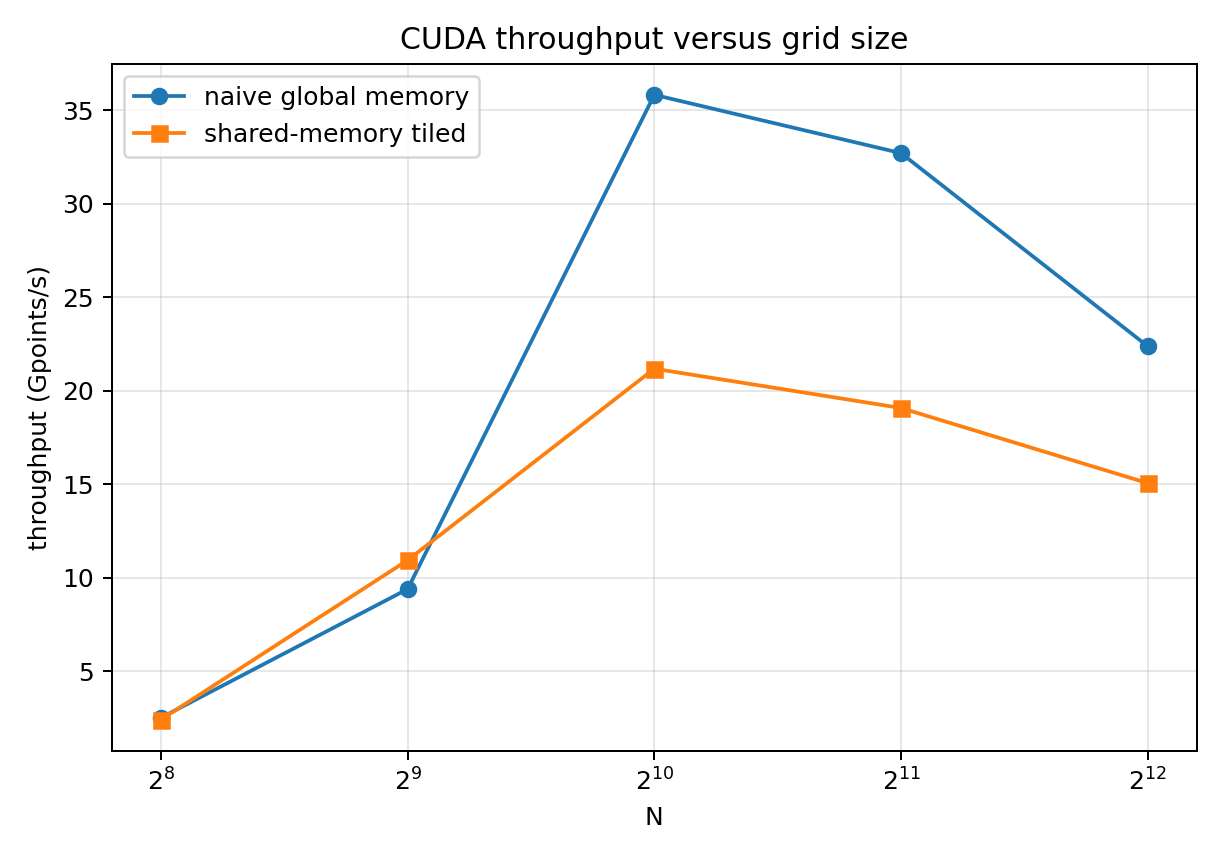
\includegraphics[width=0.80\linewidth]{plots/throughput_vs_n.png}
\caption{Throughput of the two CUDA kernels.}
\end{figure}

\begin{center}
\begin{tabular}{rrr}
\toprule
\(N\) & Naive \(8\times8\) (Gpt/s) & Shared \(16\times16\) (Gpt/s) \\
\midrule
256 & 2.511 & 2.414 \\
512 & 9.394 & 10.937 \\
1024 & 35.824 & 21.178 \\
2048 & 32.707 & 19.077 \\
4096 & 22.381 & 15.058 \\
\bottomrule
\end{tabular}
\end{center}

In this run, both selected configurations peaked at \(N=1024\). Smaller grids
do not give the GPU enough work. At larger sizes, the working set becomes less
cache-friendly and the laptop GPU is more limited by memory bandwidth and
clock/power behavior.

\section{Files}

\begin{center}
\begin{tabular}{ll}
\toprule
File & Purpose \\
\midrule
\texttt{heat\_common.hpp} & Shared CPU solver, initialization, and output helpers \\
\texttt{heat\_serial.cpp} & Serial 2D heat solver \\
\texttt{heat\_cuda.cu} & Naive CUDA solver \\
\texttt{heat\_cuda\_tile.cu} & Shared-memory CUDA solver \\
\texttt{cuda\_common.cuh} & CUDA error checking and device helpers \\
\texttt{cuda\_device\_info.cu} & Prints GPU information \\
\texttt{Makefile} & Build commands \\
\texttt{scripts/run\_benchmarks.sh} & Runs validation, timings, and plotting \\
\texttt{scripts/plot\_results.py} & Creates plots and parsed CSV files \\
\bottomrule
\end{tabular}
\end{center}

\section{Notes}

The main surprise was that my shared-memory kernel did not beat the naive
kernel. I checked both CUDA versions against the CPU code, so this does not
look like a correctness problem. The likely reason is that the naive kernel is
already cache-friendly on this GPU, while the tiled version pays extra overhead
for halo loading and synchronization.

I also avoided copying the full grid back to the host during the time loop. For
the convergence check, only the maximum update value is reduced and copied when
needed.

\end{document}
